\chapter{An�lisi de resultats}
\label{chapter:results}
En aquest cap�tol es mostren les principals proves realitzades per cadascuna de les tres parts del sistema que hem descrit als cap�tols anteriors


\section{Cerca de refer�ncies}
En primer lloc provarem com de b� ho fa el sistema a l'hora de cercar p�gines a Internet que continguin informaci� sobre un article concret. Els tests que hem dut a terme consisteixen en els passos seg�ents:
\begin{enumerate}
\item{Obtenir una s�rie de consultes d'un llistat de documents PDF}
\item{Cercar cadascuna de les consultes amb: \textit{Google}, \textit{Bing} i \textit{Yahoo}}
\item{Per cadascun dels resultats obtinguts, analitzem si �s bo o no}
\item{Comptabilitzem el n�mero de consultes que han fet falta per obtenir el primer \textit{bon} resultat}
\end{enumerate}

Noteu que per tal classificar els resultats en bons i dolents nomes comprovem si part de la informaci� que volem es troba dins de la p�gina resultant. Aquesta no �s una soluci� perfecta, per� ens permet fer una aproximaci� sobre la quantitat de fitxers pels quals en podem trobar la refer�ncia.

\paragraph{}
Una altra q�esti� sobre la implementaci� dels tests, �s que els resultats obtinguts se solen repetir entre consultes del mateix article. Per estalviar temps i evitar fer moltes peticions seguides als mateixos servidors (que podrien resultar en un bloqueig), deixem uns segons entre petici� i petici� i emmagatzemem cada resultat de manera que nom�s l'haguem de demanar una sola vegada. A m�s, en molts casos els resultats corresponen al mateix fitxer PDF del qual estem buscant informaci� i els hem d'ometre.

\paragraph{}
Les proves s'han realitzat per conjunts d'articles diferents agrupats depenent la seva cap�alera, que �s el que pot fer variar m�s els resultats obtinguts, i un �ltim grup amb articles de qualsevol tipus. Les figures \ref{fig:results:random-reslen} i \ref{fig:results:random-fqlen} a mostren els resultats d'aquest �ltim conjunt.
\begin{figure}[h!]
\begin{center}
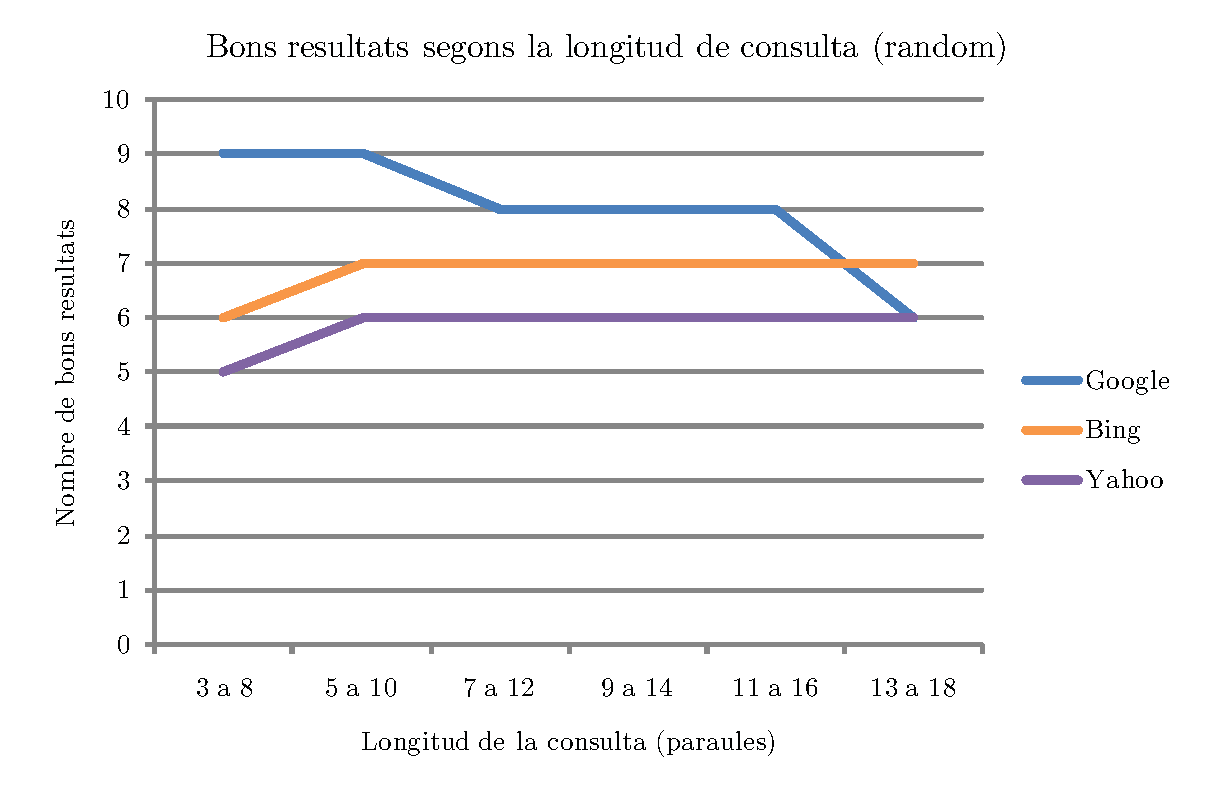
\includegraphics[width=0.9\textwidth]{figures/results:random-reslen.pdf}
\caption{Comparaci� de la qualitat dels resultats obtinguts segons la llargada de les consultes}
\label{fig:results:random-reslen}
\end{center}
\end{figure}

\paragraph{}
Tot i que en algunes ocasions els resultats bons retornats per \textit{Bing} o \textit{Yahoo} s�n superiors en nombre, en general, el cercador \textit{Google} ofereix major cobertura amb resultats sobre m�s articles.



\begin{figure}[h!]
\begin{center}
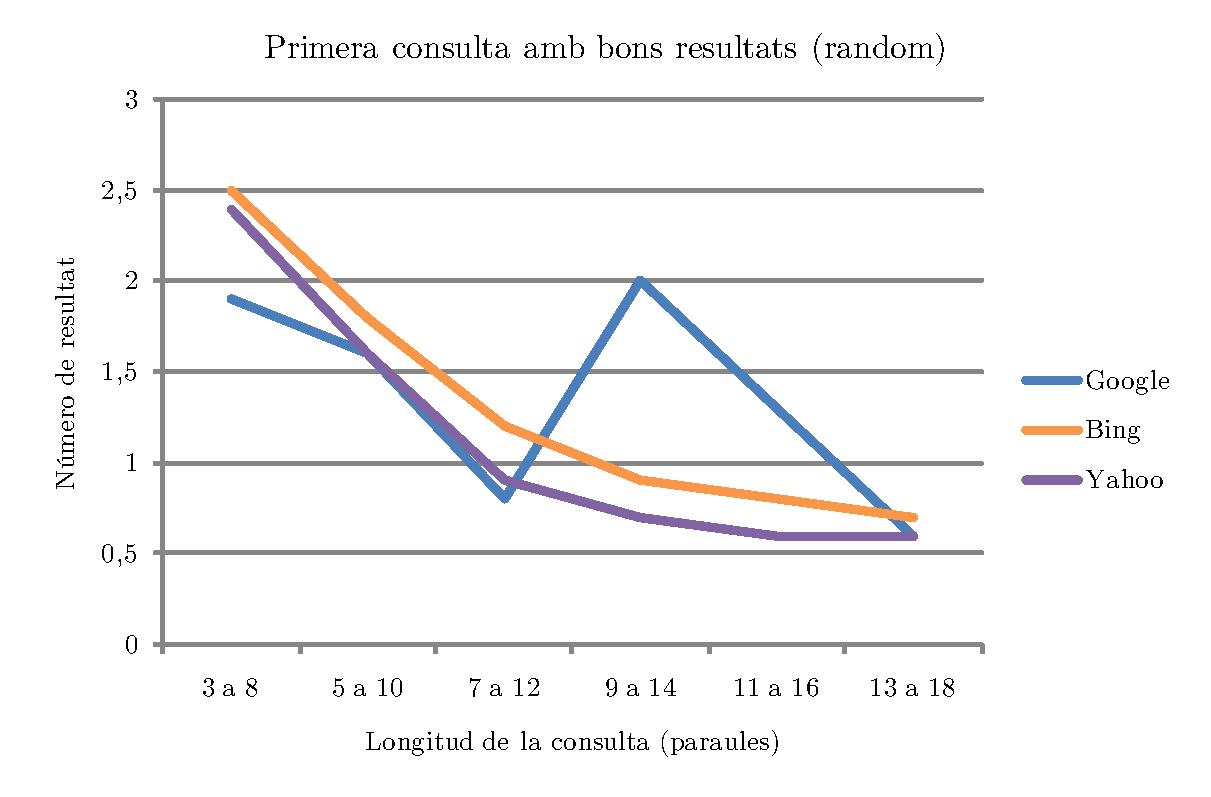
\includegraphics[width=0.9\textwidth]{figures/results:random-fqlen.pdf}
\caption{Comparaci� del n�mero de consultes necess�ries abans de trobar bons resultats}
\label{fig:results:random-fqlen}
\end{center}
\end{figure}

Finalment, respecte les consultes veiem que com mes llargues s�n, el n�mero de cerques que hem de fer per obtenir bons resultats disminueix. 

\section{Extracci� de refer�ncies}
text

\section{Inducci� de \textit{wrappers}}
text






